\section{受迫响应}
\label{sec:wave-forced}

弦上持续受力，或者端点被人摇动，解怎样由这些输入决定？线性问题的办法是把输入切成很多瞬时的小份，每一份单独算，再加起来。

\paragraph{脉冲等于初速度}
先看单个振子的例子。第~\ref{chap:linear-differential-systems}章的常数变易公式对$\ddot{x}+\omega^{2}x=g(t)$、零初值给出
\[
 x(t)=\int_0^{t}\frac{\sin\omega(t-s)}{\omega}\,g(s)\,\mathrm{d}s .
\]
被积函数中的$\sin\omega(t-s)/\omega$，是时刻$s$得到单位初速度之后，经过时间$t-s$的自由振动。外力在极短的时间$\mathrm{d}s$内提供的冲量是$g(s)\,\mathrm{d}s$，它的效果就是让速度突然增加这么多。

把振子换成弦，道理不变。时刻$s$的外力$f(\cdot,s)$在$\mathrm{d}s$内给弦增加的速度是$f(\cdot,s)\,\mathrm{d}s$，这相当于在时刻$s$从零位移出发，以这个速度分布开始一次自由振动。

\begin{theorem}[\term{Duhamel原理}（Duhamel's principle）]
\label{thm:wave-duhamel}
设$f$和$\partial_xf$在$\mathbb{R}\times[0,T]$上连续。对每个$s\in[0,T]$，记$w(\cdot,\cdot\,;s)$是自由波动方程在$t\geq s$上的解，它在时刻$s$的位移为零，速度为$f(\cdot,s)$。则
\begin{equation}
 u(x,t)=\int_0^{t}w(x,t;s)\,\mathrm{d}s=\frac1{2c}\int_0^{t}\int_{x-c(t-s)}^{x+c(t-s)}f(y,s)\,\mathrm{d}y\,\mathrm{d}s
 \label{eq:wave-duhamel}
\end{equation}
是$\partial_t^{2}u-c^{2}\partial_x^{2}u=f$在零初值下的$C^{2}$解。
\end{theorem}

\begin{proof}
由式~\eqref{eq:wave-dalembert}，从时刻$s$算起，$w$的表达式为
\[
 w(x,t;s)=\frac1{2c}\int_{x-c(t-s)}^{x+c(t-s)}f(y,s)\,\mathrm{d}y .
\]
它给出式~\eqref{eq:wave-duhamel}的第二个等号。直接求导，$\partial_tw$是$f$在两端点处值的平均，$\partial_t^{2}w$和$\partial_x^{2}w$都由$\partial_xf$在端点的值表示。这些导数对$(x,t,s)$连续，可以在积分号下求导。

对$t$求一次导，积分上限带来一项$w(x,t;t)$。这一项的积分区间长度为零，所以等于零：
\[
 \partial_tu(x,t)=w(x,t;t)+\int_0^{t}\partial_tw(x,t;s)\,\mathrm{d}s=\int_0^{t}\partial_tw(x,t;s)\,\mathrm{d}s .
\]

再求一次导，上限这次带来$\partial_tw(x,t;t)$，按定义它等于$f(x,t)$：
\[
 \partial_t^{2}u=f(x,t)+\int_0^{t}\partial_t^{2}w\,\mathrm{d}s=f(x,t)+c^{2}\int_0^{t}\partial_x^{2}w\,\mathrm{d}s=f+c^{2}\partial_x^{2}u .
\]
令$t=0$，由上面两式得$u(\cdot,0)=0$，$\partial_tu(\cdot,0)=0$。
\end{proof}

定理对$f$的光滑性要求来自$\partial_x^{2}w$要由$\partial_xf$表示。$f$只是连续甚至只是局部可积时，式~\eqref{eq:wave-duhamel}仍有意义，它给出的是弱解，下面持续施力的例子就属于这种情形。一般的初值问题由线性性得到：式~\eqref{eq:wave-dalembert}加上式~\eqref{eq:wave-duhamel}。

\paragraph{外力的依赖区域}
式~\eqref{eq:wave-duhamel}的积分区域是点$(x,t)$的回溯三角形，如图~\ref{fig:wave-duhamel}(a)。时刻$s$的外力只在宽度$2c(t-s)$的切片上起作用，越接近$t$，切片越窄。

三角形内的权重处处是常数$1/(2c)$。换个角度看图~\ref{fig:wave-duhamel}(b)：在点$(y,s)$施加单位脉冲，此后的响应在前向锥内是$1/(2c)$，锥外是零。这是实轴上的Green函数，用公式写是
\begin{equation}
 G(x,t;y,s)=\frac1{2c}\,\mathbb{I}\{\lvert x-y\rvert<c(t-s)\}.
 \label{eq:wave-green}
\end{equation}
式~\eqref{eq:wave-duhamel}就是用$G$对$f$积分。

\begin{BookInlineFigure}
  \centering
  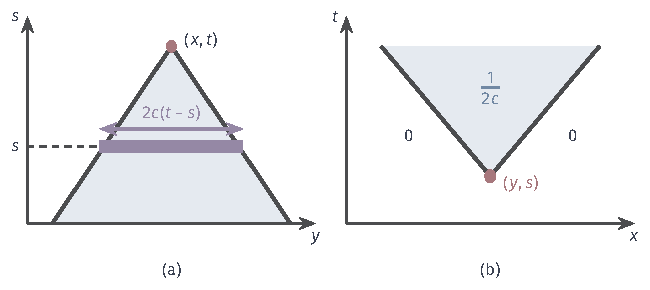
\includegraphics[width=110.06mm]{figures/06-differential-equations/02-partial-differential-equations/tikz/wave-duhamel/figure.pdf}
  \caption{外力的作用范围。(a)计算$u(x,t)$要积分回溯三角形内的$f$，紫色条带是时刻$s$的切片，宽度为$2c(t-s)$。(b)点$(y,s)$（红）的单位脉冲只在前向锥内产生响应，值为$1/(2c)$，锥外为零。}
  \label{fig:wave-duhamel}
\end{BookInlineFigure}

\paragraph{瞬时冲击与持续驱动}
比较两种施力方式，取$c=1$。一种是$t=0$时的一次单位冲击，相当于初速度$\mathbb{I}\{\lvert x\rvert<1\}$，第~\ref{sec:wave-dalembert}节已算出$u(0,t)=\min\{t,1\}$。另一种是在同一区间上持续施力，$f=\mathbb{I}\{\lvert x\rvert<1\}$对所有$t\geq0$成立。

持续驱动相当于每一时刻都敲一次。由式~\eqref{eq:wave-duhamel}，时刻$s$的那一次敲击到$t$时在$x=0$的贡献是$\min\{t-s,1\}$。令$r=t-s$，积分得到
\[
 u(0,t)=\int_0^{t}\min\{r,1\}\,\mathrm{d}r=
 \begin{cases}
  t^{2}/2, & 0\leq t\leq1,\\
  t-\frac12, & t\geq1.
 \end{cases}
\]

例如$t=1$时$u(0,1)=1/2$，$t=3$时$u(0,3)=5/2$。一次冲击的响应到$t=1$后不再变化；持续驱动的响应在$t>1$后线性增长，因为不断有新的敲击的贡献抵达这一点。

图~\ref{fig:wave-impulse-sustained}(a)显示持续驱动如何由各次冲击累加：浅色的梯形是时刻$s=2,1,0$的单次冲击到$t=3$时的响应，蓝色的钟形是所有时刻的积分。(b)是两种情形在原点处的时间历程。

\begin{BookInlineFigure}
  \centering
  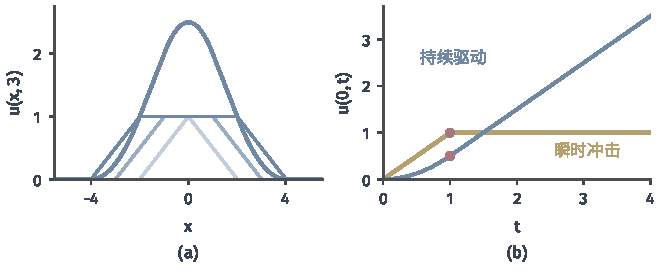
\includegraphics[width=112mm]{figures/06-differential-equations/02-partial-differential-equations/matplotlib/wave-impulse-sustained/figure.pdf}
  \caption{瞬时冲击与持续驱动，$c=1$，力作用在$(-1,1)$上。(a)$t=3$时的位移：蓝色由浅到深的三个梯形是时刻$s=2,1,0$的单次冲击的响应，粗蓝线是持续驱动的解，等于全部冲击响应的积分。(b)原点处的位移，黄线是一次冲击，蓝线是持续驱动，红点是$t=1$时的值$1$和$1/2$。}
  \label{fig:wave-impulse-sustained}
\end{BookInlineFigure}

\paragraph{有限区间：逐模式受迫与共振}
在$(0,L)$上两端固定，把解按式~\eqref{eq:wave-dirichlet-modes}的模式展开，每个系数$a_n(t)$都是一个受迫振子。设$f_n(t)$是$f(\cdot,t)$的正弦系数，零初值时
\begin{equation}
 \ddot{a}_n+\omega_n^{2}a_n=f_n(t),\qquad a_n(t)=\int_0^{t}\frac{\sin\omega_n(t-s)}{\omega_n}f_n(s)\,\mathrm{d}s .
 \label{eq:wave-modal-forcing}
\end{equation}

取$L=1$，$c=1$，$f=\sin(\pi x)\cos(\Omega t)$，只有第一个模式被驱动，固有频率是$\omega_1=\pi$。$\Omega\neq\pi$时，解是特解加上消去初值的齐次解：
\[
 a_1(t)=\frac{\cos\Omega t-\cos\pi t}{\pi^{2}-\Omega^{2}} .
\]
它一直有界。例如$\Omega=2$时，$\lvert a_1\rvert\leq2/(\pi^{2}-4)\approx0.34$。

当$\Omega=\pi$时，上式的分母为零。令$\Omega\to\pi$取极限，由L'Hôpital法则得到
\[
 a_1(t)=\frac{t\sin\pi t}{2\pi} .
\]
代入方程可以验证：$\ddot{a}_1=\cos\pi t-\pi^{2}a_1$。幅度随时间线性增长，这就是共振：外力每个周期都在弦运动的方向上推，能量持续积累。

对比热方程的同一模式。$\dot{a}+\pi^{2}a=\cos\pi t$的解是一个有界的振荡加上快速衰减的暂态，幅度约为$1/(\pi\sqrt{\pi^{2}+1})\approx0.096$。扩散会不断耗掉输入，所以没有共振。图~\ref{fig:wave-resonance}对比了这三种响应。

\begin{BookInlineFigure}
  \centering
  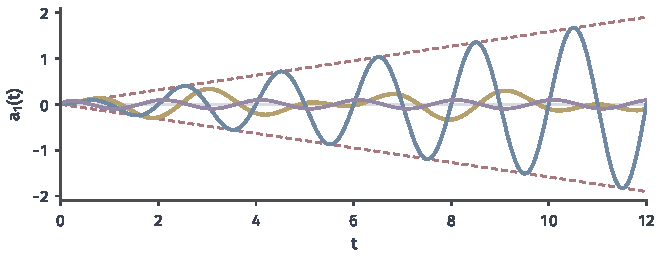
\includegraphics[width=112mm]{figures/06-differential-equations/02-partial-differential-equations/matplotlib/wave-resonance/figure.pdf}
  \caption{第一个模式在外力$\cos\Omega t$下的响应，$L=1$，$c=1$。蓝线是共振$\Omega=\pi$，红色虚线是它的包络$\pm t/(2\pi)$。黄线是非共振$\Omega=2$。紫线是热方程同一模式在$\Omega=\pi$下的响应。}
  \label{fig:wave-resonance}
\end{BookInlineFigure}

\paragraph{边界输入与能量}
除了体内的外力，也可以摇动端点。考虑半直线$x>0$，初值为零，左端按$u(0,t)=g(t)$运动，并设$g(0)=g'(0)=0$。此时右行波$u=g(t-x/c)$满足方程，并在$x=0$处取$g(t)$，所以解是
\begin{equation}
 u(x,t)=
 \begin{cases}
  g(t-x/c), & 0\leq x<ct,\\
  0, & x\geq ct .
 \end{cases}
 \label{eq:wave-boundary-solution}
\end{equation}
端点的运动沿特征线原样传到各处，只是延迟了$x/c$。

由式~\eqref{eq:wave-end-power}，端点的输入要算入能量账。这里$\partial_tu=g'$，$\partial_xu=-g'/c$，端点$x=0$的外法向导数是$-\partial_x$。把$\kappa$换成$c^{2}$（即除以线密度$\rho$），单位质量的输入功率是
\[
 P(t)=c^{2}\cdot\frac{g'(t)}{c}\cdot g'(t)=c\,g'(t)^{2}.
\]
弦原本静止时，摇动端点总在向弦输入能量，功率与端点速度的平方成正比，与$g$的符号无关。

取$c=1$，$g(t)=\sin^{2}\pi t$（$0\leq t\leq1$），此后$g=0$。这里$g'(t)=\pi\sin2\pi t$，$g''$在$t=0,1$有跳跃，所以解的二阶导数在两条特征线$x=t$和$x=t-1$上跳跃，其他位置方程按经典意义成立。累计输入的能量是
\[
 \int_0^{1}P(t)\,\mathrm{d}t=\int_0^{1}\pi^{2}\sin^{2}2\pi t\,\mathrm{d}t=\frac{\pi^{2}}2\approx4.93 .
\]

弦上的能量可以独立算一遍来核对。$t\geq1$时，由式~\eqref{eq:wave-boundary-solution}，$\partial_tu$和$\partial_xu$的平方都等于$g'(t-x)^{2}$，所以
\[
 E(t)=\frac12\int_0^{\infty}\bigl[(\partial_tu)^{2}+(\partial_xu)^{2}\bigr]\,\mathrm{d}x=\int_0^{1}g'(r)^{2}\,\mathrm{d}r=\frac{\pi^{2}}2 .
\]
两种算法结果相同，能量在端点停止摇动后保持不变，如图~\ref{fig:wave-boundary-drive}。

\begin{BookInlineFigure}
  \centering
  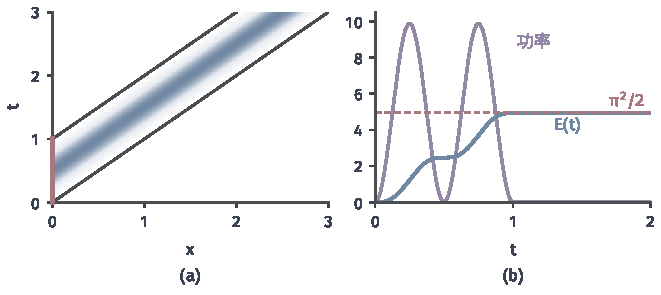
\includegraphics[width=112mm]{figures/06-differential-equations/02-partial-differential-equations/matplotlib/wave-boundary-drive/figure.pdf}
  \caption{端点驱动的半直线，$c=1$，$g(t)=\sin^{2}\pi t$（$0\leq t\leq1$，红色粗线）。(a)时空热图：端点的运动沿特征线传播，深灰直线是波包的前后沿。(b)输入功率$g'(t)^{2}$（紫）和弦上的能量$E(t)$（蓝，由空间积分算出），红色虚线是总输入$\pi^{2}/2$。}
  \label{fig:wave-boundary-drive}
\end{BookInlineFigure}

有限区间上，非齐次的边界条件可以转移成外力。若$u(0,t)=g(t)$，$u(L,t)=0$，令$R(x,t)=g(t)(1-x/L)$，$v=u-R$。$v$在两端为零，满足下面的方程，初值相应地减去$R$和$\partial_tR$在$t=0$的值：
\[
 \partial_t^{2}v-c^{2}\partial_x^{2}v=f-g''(t)\Bigl(1-\frac xL\Bigr).
\]
这样就回到了逐模式受迫的情形。此时端点的功率不一定为正，因为反射回来的波可以推动端点，把能量还给驱动源。
